Chaque sommet de $G_{k,k'}$ est identifi\'e par le couple $(i,j)$ avec $0 \le i < k$ et $0 \le j < k'$. Le sommet $(i,j)$ est adjacent  au sommet :
\begin{itemize}
	\item $(i, j+1)$ si $j < k'-2$
	\item $(i+1,j)$ si $i < k-2$
	\item $(i,j-1)$ si $j > 0$
	\item $(i-1,j)$ si $i > 0$
\end{itemize}
De plus, les sommets  $(0,0)$ et $(0,k-1)$,  $(0,0)$ et $(0,k'-1)$ , $(k-1,0)$ et $(k-1,k'-1)$, $(0,k'-1)$ et $(k-1,k'-1)$ sont adjacents.
On remarque que tout graphe  induit par un sommet et son voisinage forme un graphe \'etoile $K_{1,4}$.
La figure \ref{exempleGrapheCellule} est un exemple de {\em grille boucl\'ee} $G_{4,4}$. Ce graphe contient $16$ sommets, $28$ ar\^etes. Les sommets $(0,0), (0,1), (1,1), (1,0)$ forme une cellule et le graphe $G_{4,4}$ contient  $10$ cellules. 
% ---- figure exemple graphe cellule G_{4,4}
\begin{figure}[htb!] 
\centering
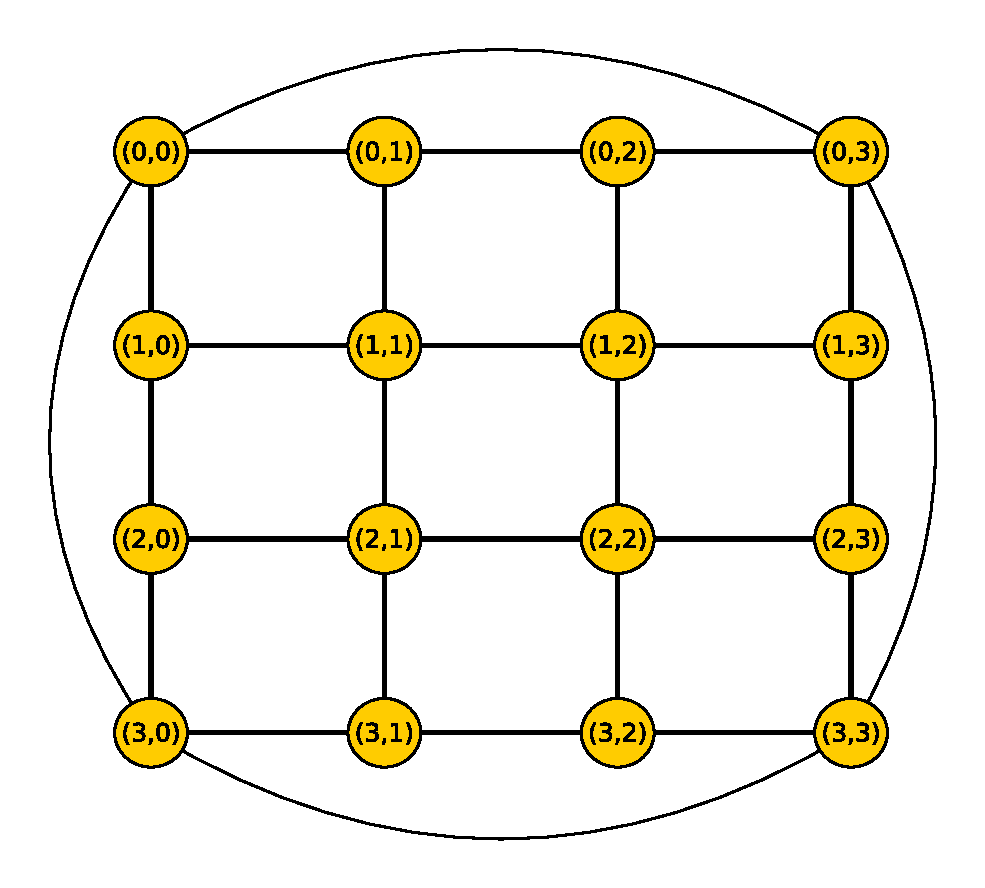
\includegraphics[scale=0.6]{exempleGrapheCelluleG33.eps}
\caption{ La grille boucl\'ee $G_{4,4}$ : elle est compos\'ee de $16$ sommets, $28$ ar\^etes et $10$ cellules. }
\label{exempleGrapheCellule} 
\end{figure}
%\FloatBarrier
% ---- figure exemple graphe cellule G_{4,4}
\begin{definition}
Une cellule est un cycle de longueur $4$ identifi\'e par les sommets $(i,j)$, $(i,j+1)$, $(i+1,j)$ et $(i+1,j+1)$ avec $i<k-1$ et $j<k'-1$. Nous notons une telle cellule $C_{i,j}$.
\end{definition}
Si $k = k' = 2$, la grille boucl\'ee $G_{2,2}$ est la cellule $C_{0,0}$.

\begin{property}
Le graphe $G_{k,k'}$ poss\`ede $k \times k'$ sommets,  $k \times (k'-1) + k' \times(k-1) + 4$  ar\^etes et $k \times k' +1$ cellules.
\end{property}
